\subsection{Our Approach} 




Fig.~\ref{fig:overallarchitecture} shows an overview of our approach. Given a function and an optional verification goal, the objective is to automatically generate loop invariants and function pre-/postconditions. If a verification goal is provided, these specifications should be sufficient to prove it; otherwise, they should capture useful functional relations exposed by the available symbolic states.
Following the three design choices of Section~\ref{sec:intro}, symbolic execution drives the pipeline and computes path-sensitive symbolic information at the current boundary; \toolname\ injects these facts into invariant templates and ACSL skeletons, while a lightweight static route selects supporting examples and ACSL guidance. The LLM therefore receives both semantic facts from the current symbolic state and prompt support material matched to the program's syntactic features. The verifier then checks the candidate, and if it fails, the parsed verifier feedback is combined with the same local symbolic context to drive iterative refinement until a verifier-checked summary is produced. Each generation call is issued at a symbolic-execution boundary --- a loop, an unspecified callee, a recursive data structure, or a recursive function --- and once a verifier-checked summary is obtained, symbolic execution resumes from the same point using that summary.

 

 
Fig.~\ref{fig:overallarchitecture} divides function-specification generation into four symbolic-execution-driven stages and an LLM fallback (Section~\ref{sec:llm-fallback}) for self-recursion, recursive data structures, external calls, path explosion, floating-point arithmetic, and runtime errors. The first stage, \textbf{Default Precondition Generation}, creates memory-safety conditions for symbolic execution (node \circled{0} in Fig.~\ref{fig:example}); Section~\ref{sec:default-pre} gives the details.
 

From the default precondition, symbolic execution starts at function entry (node \circled{1} in Fig.~\ref{fig:example}). At a call (node \circled{2}), \toolname\ pauses to recursively generate the callee specification (nodes \circled{3}--\circled{6}), then applies that contract at the call site and resumes the caller. A call stack handles nested calls; generated specifications are stored for reuse, yielding bottom-up processing.



\begin{figure}[!t]
    \centering
    \begin{tikzpicture}
      \node[inner sep=0pt] (overviewfig) {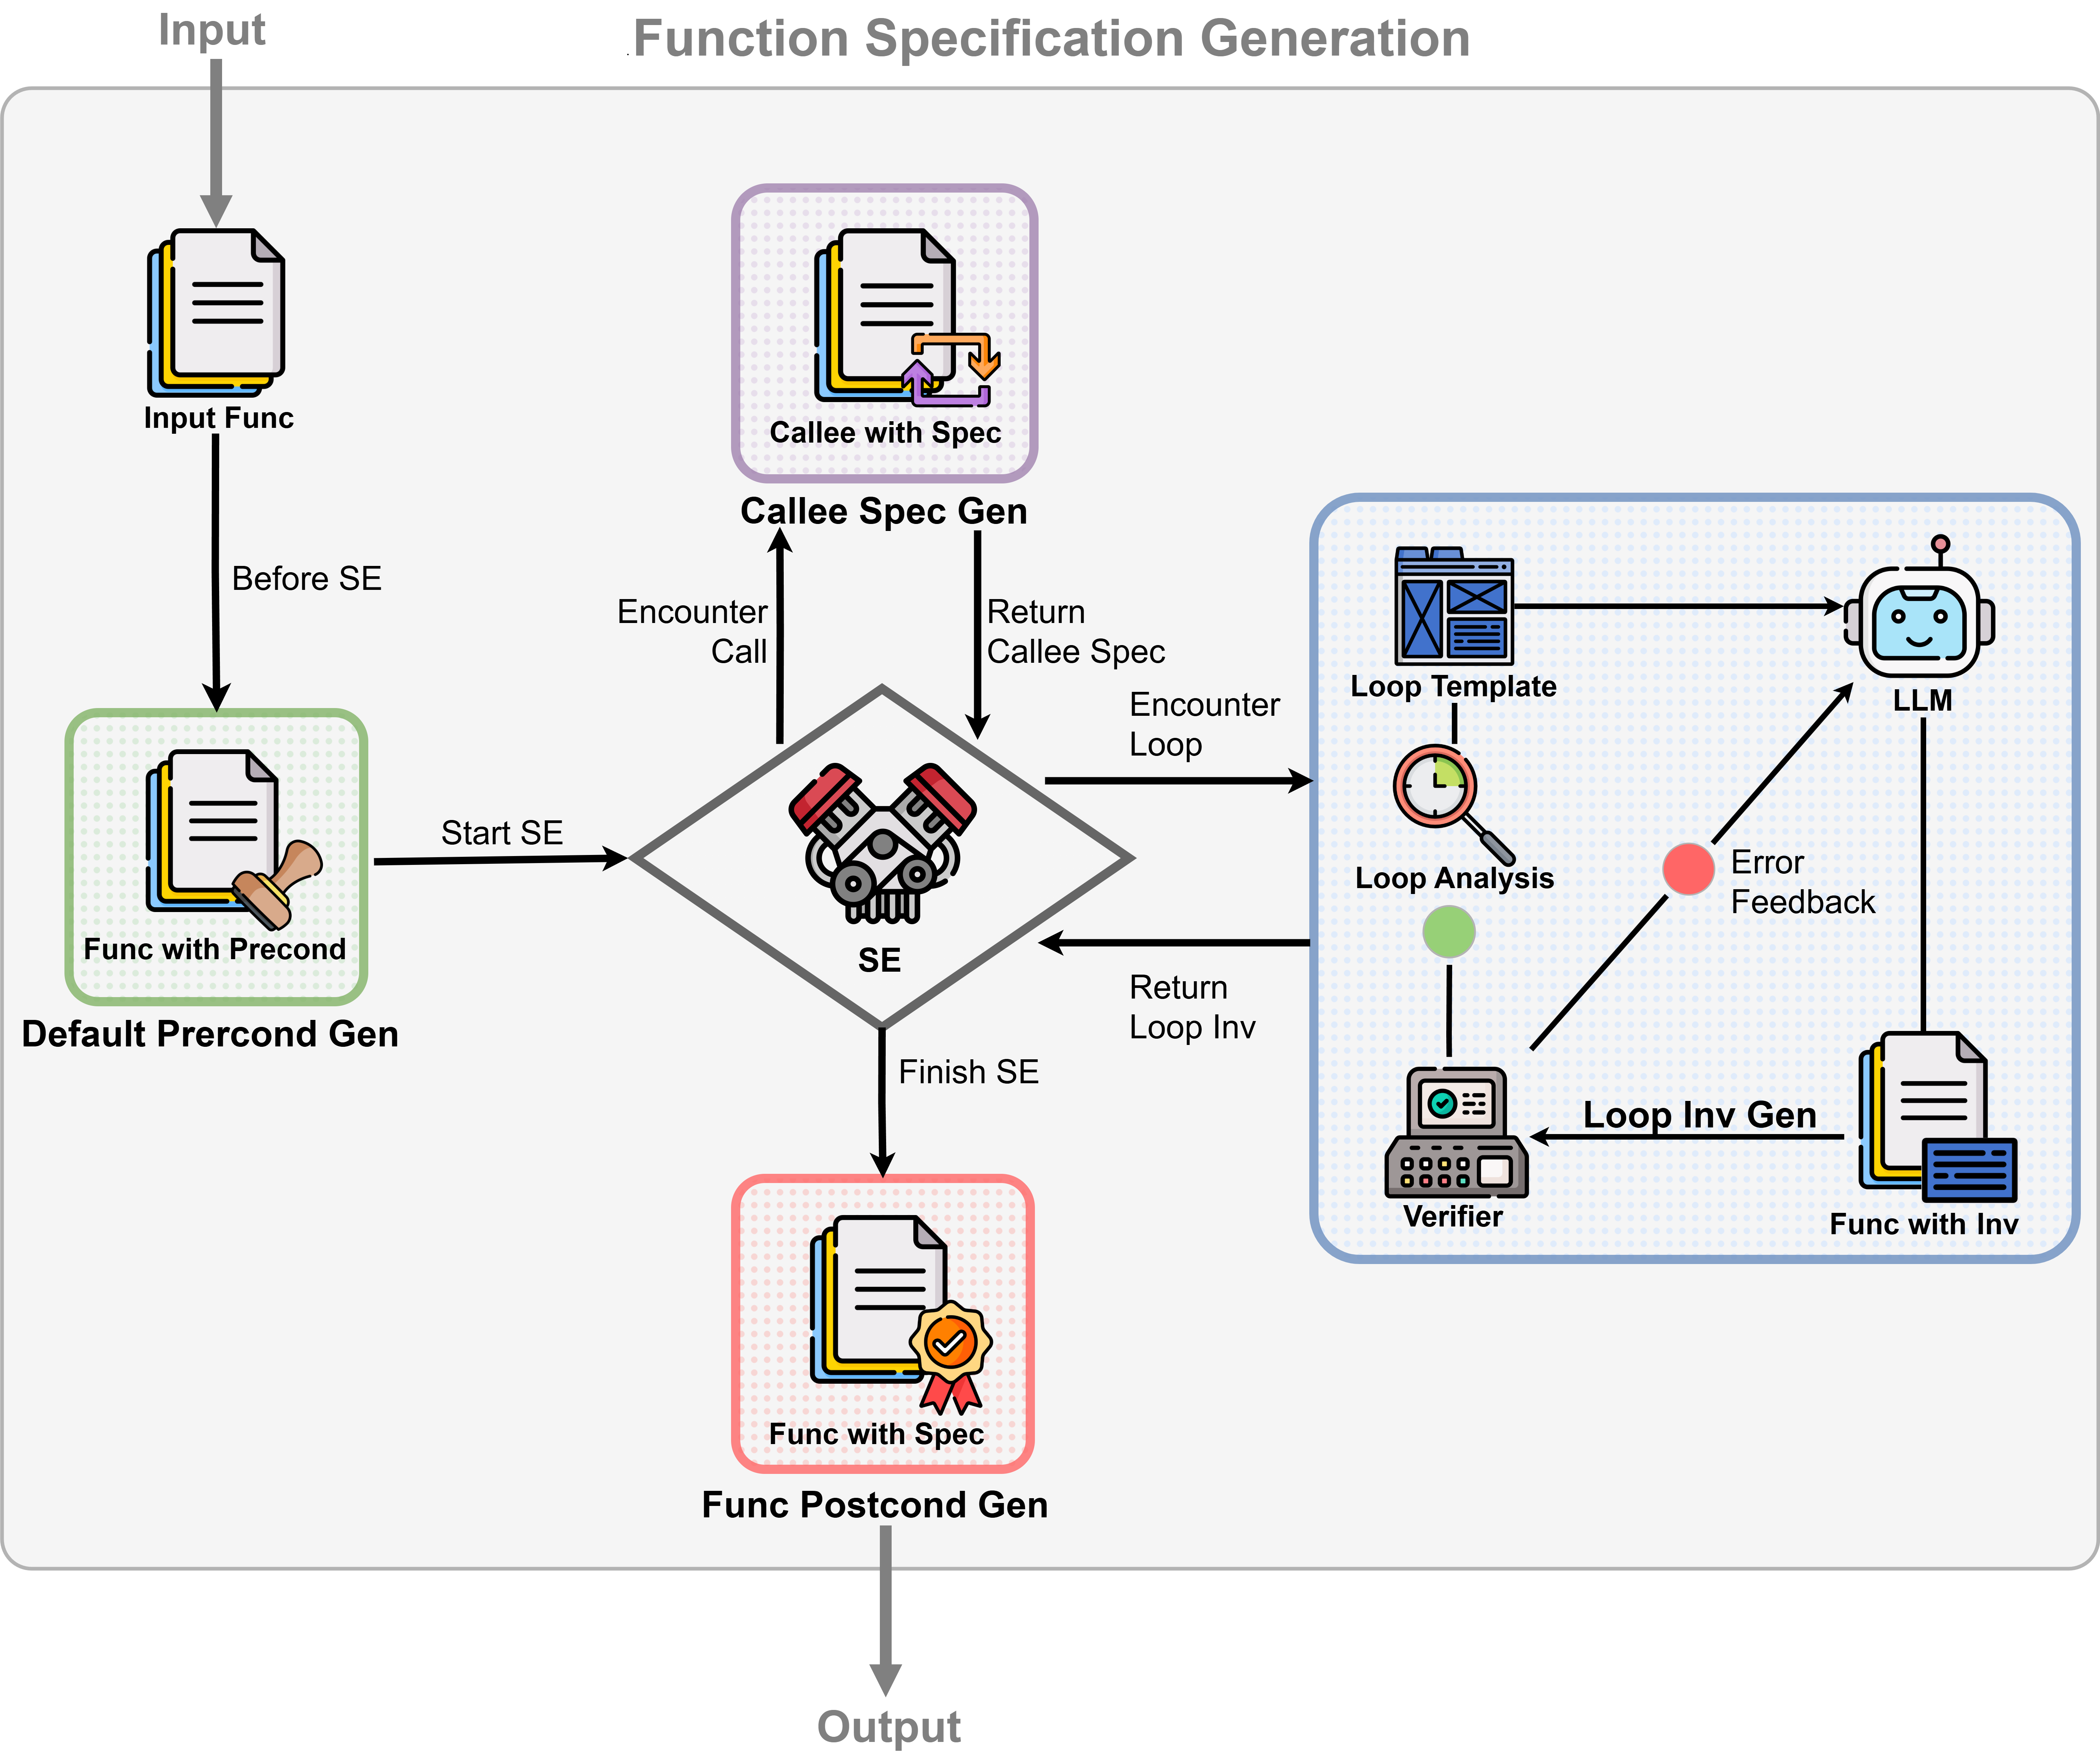
\includegraphics[width=\columnwidth]{images/overview.png}};
      \fill[white,opacity=0.16] (overviewfig.south west) rectangle (overviewfig.north east);
    \end{tikzpicture}
    \caption{Overview of Our Approach}
    \label{fig:overallarchitecture}
\end{figure}

At a loop (node \circled{5} in Fig.~\ref{fig:example}), symbolic execution pauses for \textbf{Loop Invariant Generation}. Loop Analysis uses the entry state and body to identify unchanged variables (\texttt{pIp->len}, \texttt{pIp}, \texttt{pIp->pkv}) and inductive variables (\texttt{i}, \texttt{chksum}). It records the guard \texttt{i < pIp->len} and the condition for at least one iteration, \texttt{0 < \textbackslash at(pIp, Pre)->len}. These facts instantiate ACSL templates with guards, frame clauses, and relation placeholders, illustrated below (the complete annotations appear in Fig.~\ref{fig:example}).


{
\footnotesize
\[
\begin{array}{@{}l@{}}

  \texttt{loop invariant} \texttt{(0 < \textbackslash at(pIp, Pre)->len)} \\
  \quad \texttt{==> PLACE\_HOLDER\_for\_i;} \\
  \texttt{loop invariant} \texttt{(0 < \textbackslash at(pIp, Pre)->len)} \\
  \quad \texttt{==> PLACE\_HOLDER\_for\_chksum;} \\
  \texttt{loop invariant pIp == \textbackslash at(pIp, Pre);}

\end{array}
\]
}
These skeletons provide specific \texttt{PLACE\_HOLDER} tags for the LLM to populate (marked as the blue boxes in Fig.~\ref{fig:example}). Guided by these structured templates and symbolic execution results,
the LLM produces loop invariants that capture useful relations among different types of variables. This symbolic-state-guided structure narrows the candidate space and makes key logical constraints explicit before the LLM fills the placeholders. For instance, the generated invariants correctly incorporate the loop-entry condition \texttt{(0 < \textbackslash at(pIp, Pre)->len)}---the critical logical constraint whose omission caused the pure-LLM failures in Section~\ref{sec:motivation}.

During Loop Invariant Generation, the verifier-guided refinement procedure is iteratively invoked to assess both the validity of the generated invariants and their usefulness for proving the given verification goal when such a goal is available. Depending on verifier feedback, different refinement strategies guide the LLM toward verifier-checked invariants. 

When symbolic execution of the callee is completed (node \circled{6} in Fig.~\ref{fig:example}), \textbf{Function Postcondition Generation} (marked in red in Fig.~\ref{fig:overallarchitecture}) is triggered. The resulting symbolic states are used to synthesize a postcondition that summarizes the callee's functional behavior. Upon completion, the generated pre-/postconditions are returned to the call site and reused as a functional summary in the caller (node \circled{7} in Fig.~\ref{fig:example}), enabling symbolic execution of the caller to resume without re-analyzing the callee's internal control flow. 







This example illustrates the full pipeline; goal-independent generation is evaluated separately in Section~\ref{sec:large-scale-experiment}.
